% style notes
% - \,percent not \%

\documentclass[12pt, preprint]{aastex}

% words
\newcommand{\project}[1]{\textsl{#1}}
\newcommand{\thecannon}{\project{The~Cannon}} 
\newcommand{\tc}{\project{The~Cannon}} 
\newcommand{\apogee}{\project{APOGEE}}
\newcommand{\apokasc}{\project{APOKASC}}
\newcommand{\aspcap}{\project{ASPCAP}}
\newcommand{\corot}{\project{Corot}}
\newcommand{\kepler}{\project{Kepler}}
\newcommand{\gaia}{\project{Gaia}}
\newcommand{\gaiaeso}{\project{Gaia--ESO}}
\newcommand{\galah}{\project{GALAH}}
\newcommand{\most}{\project{MOST}}
\newcommand{\code}[1]{\texttt{#1}}
\newcommand{\documentname}{\textsl{Article}}

\newcommand{\teff}{\mbox{$\rm T_{eff}$}}
\newcommand{\kms}{\mbox{$\rm kms^{-1}$}}
\newcommand{\feh}{\mbox{$\rm [Fe/H]$}}
\newcommand{\xfe}{\mbox{$\rm [X/Fe]$}}
\newcommand{\alphafe}{\mbox{$\rm [\alpha/Fe]$}}
\newcommand{\mh}{\mbox{$\rm [M/H]$}}
\newcommand{\logg}{\mbox{$\rm \log g$}}
\newcommand{\noise}{\sigma_{n\lambda}}
\newcommand{\scatter}{s_{\lambda}}
\newcommand{\pix}{\mathrm{pix}}
\newcommand{\rfn}{\mathrm{ref}}
\newcommand{\rgc}{\mbox{$\rm R_{GC}$}}
\newcommand{\vgal}{\mbox{$\rm V_{GAL}$}}

% math
\newcommand{\numax}{$\nu_{\max}$}
\newcommand{\deltanu}{$\Delta\nu$}

\begin{document}

% To do. 
% 1. release two catalogues :
% 1a) trained on log mass and 1b) trained on log mass
%2. resample the errors in label space - add a random error to the mass term and rerun the labels through the cannon and see if the standard deviation and bias in the take one out test is any different - if not we know the noisiness in the training set is not an issue
%3. cut out a lot of regions except for the CN and retrain and see if the take-out-out test sigma increases or decreases in the dispersion - if increases we know we are limited by the information available in the data. If decreases there is degeneracy / noisiness in the covariance of labels? 

% plotting in /Apogee_ages/makeplot_scatter_test18_step.py 
% and plotelements_on_spectra.py 

\title{Measuring red-giant masses and ages with stellar spectra}
\author{M.~Ness\altaffilmark{1},
David~W.~Hogg\altaffilmark{1,2,3},
H.-W.~Rix\altaffilmark{1},
\textbf{others}}
\altaffiltext{1}{Max-Planck-Institut f\"ur Astronomie, K\"onigstuhl 17, D-69117 Heidelberg, Germany}
\altaffiltext{2}{Center for Cosmology and Particle Physics, Department of Phyics,
             New York University, 4 Washington Pl., room 424, New York, NY, 10003, USA}
\altaffiltext{3}{Center for Data Science, New York University, 726 Broadway, 7th Floor, New York, NY 10003, USA}
% \altaffiltext{4}{NSF Astronomy and Astrophysics Postdoctoral Fellow}
% \altaffiltext{5}{Department of Physics \& Astronomy, Johns Hopkins University, Baltimore, MD, 21218, USA}
\email{ness@mpia.de}

\begin{abstract}%
% Context
With \thecannon, we have demonstrated that it is possible to use a
small training set of stars with noisy spectral data and known
stellar-parameter labels to build a data-driven probabilistic model of
stellar spectra that can be used to infer stellar-parameter labels for
other stars (with differently noisy spectral data).
% Aims
% Method
Here we train this system using stars with known stellar mass labels
obtained from a training set of stars with both
\kepler\ asteroseismological observations (hence the known masses) and
\apogee\ infrared spectral data.
We find that (after training) \thecannon\ can infer stellar
masses---and therefore also stellar ages---for red-giant stars using
infrared spectral data alone.
We produce mass and inferred age labels for all XXX,000 red-giant stars in \apogee\ DR12 and show the age trends in the Milky Way for the \apogee\ red clump sample, which have small ($\approx$ distance errors).
% Results
We demonstrate the validity of the stellar masses and ages by three
methods:
Cross-validation demonstrates that the method obtains (log) mass accuracies of approximately 0.08~dex and (log) age accuracies
of roughly 0.25~dex for typical-quality \apogee\ spectra.
Second, we find that the spectral mass (or age) indicators
discovered by \thecannon\ are associated with elements that can be ``dredged up'',
specifically the CN regions of the spectra.
Third, we show that the ages of stellar structures in the
Milky Way follow gross expectations, even conditioned on abundances.
All three of these tests show that we can obtain red-giant mass and
age information from stellar spectra; these capabilities open up new
opportunities for Milky Way and stellar astrophysics.
\end{abstract}

\keywords{%
keywords: incomplete (DWH)!
---
methods: data analysis
---
methods: statistical
---
stars: abundances
---
stars: fundamental parameters
---
surveys
---
techniques: spectroscopic
}

\section{Introduction}\label{sec:Intro}

Asteroseismology surveys, such as \most, \corot, and \kepler, have
been extremely successful and productive in bringing us information
about stellar interiors and (therefore) ages.
These missions operate by taking high-cadence, high-precision stellar
photometry, in which stellar oscillation modes are visible in the
Fourier domain.
These missions have operated by taking long stretches of
uninterrupted, uniform, dense imaging data on thousands of individual
stars.
They are expensive missions, but absolutely critical to calibrate
physical stellar interior models and set standards for stellar
parameter estimation, all of which is required for the ultimate
success of the next generation of stellar surveys, particularly
including the \gaia\ Mission.

At the same time, there are many large spectroscopic surveys, such
as \apogee, \galah, and \gaiaeso, underway to measure the properties
of stellar \emph{exteriors}.
These surveys will take high signal-to-noise, high resolution spectra
of hundreds of thousands of stars, revealing detailed surface chemical
abundances.
One question that naturally arises is:
How do we use these two pieces of information (surface spectroscopy
and interior asteroseismology) to jointly infer stellar properties?
Another is:
Is there any way we could learn about stellar interiors from surface
spectroscopy?
After all, the marginal cost of taking a spectrum of
a new star is very low relative to the marginal cost of getting its
asteroseismology.

There are a small handful of specific metrics that have been used for inferring age information from surface spectroscopy alone. These derive from rotation, in the line-profile variations due to non-LTE effects, as convection scales with mass, and from chromospheric emission from a time-dependent magnetic field e.g. the Ca II HK and H$\alpha$ (see Soderblom 2010 for a review). The decay of long lived isotopes such as Th, which can be measured at 4019 Angstroms, can also be used for age dating by comparing the abundance of the long lived isotopes to that of the stable elements in the stellar photosphere. 

Importantly, and in general, mass and therefore inferred age might only appear in the spectra as
certain combinations of surface abundances that are highly covariant
with age.  For example, older stars in the Milky Way tend to be more
alpha-enhanced.  We will consider such age indicators illegitimate;
the purpose of this project is to obtain estimates for ages and masses \emph{that work even within narrow abundance-selected subsamples}.

Typically, age estimates for stars are more commonly determined not from spectroscopy directly, but from their measured stellar parameters (determined from high resolution stellar spectroscopy) by interpolating between stellar isochrone models, in the sub-giant and main sequence regime  (e.g. Bensby2013, Casagrande2011, Haywood20XX). In this \teff-\logg\ regime the models are the least insensitive to age.  However, the age constraints using this method are typically weak or may only provide an upper limit on the age estimate.  This method has been used to determine ages for what has been up until now the largest homogeneous data set of stellar ages in the galactic disk, from the Geneva Cophenhagen Survey (GCS). All of the 16,682 main sequence stars from GCS are located in the solar neighbourhood (Nordstr�m et al. 2004).

If we can determine the interior properties of stars from surface
spectroscopy alone, even noisily, great opportunities arise for
studying the stellar populations of the Milky Way and their formation. The red clump sample alone from \apogee\ alone, for which accurate distances (to 5 percent) have been determined, comprises 20,000 stars \citep{Bovy2014} and spans a radial extent across the disk of 4 -- 16 kpc. We use \tc\  \citep{Ness2015} to infer stellar masses for stars given a training set of \apokasc\ stars with known mass labels. We present our catalogue of mass and inferred ages for the 20,000 red clump stars, as well as XXXX giant stars in the DR12 data release from the \apogee\ survey. 

%We show that the spectroscopic  information informing the masses and other labels, as identified by \tc\ is in line with expectations of chemical evolution and stellar physics and we demonstrate that the mass and inferred age labels that are determined provide an additional dimension of information (that is, our age measurement does not reflect a proxy for alpha/Fe). 

%, with a sample of about 16,682 stars, has been the largest sample of stars, all of which are nearby main sequence stars, with complete data on stellar ages in the Milky Way disk. These ages have been determined from the constraints set by the measured parallaxes to these stars and their stellar parameters of \teff, \logg\ and \feh,  using interpolation between stellar isochrone models \citet{Holm2009}.



%We similarly use stellar models but determine our mass directly from the spectra - and use the models to move from measured inferred mass to inferred age. Not mapping from stellar params to isochrone age space. How do I say this in a better way to describe why it is better? 



%Skumanich 1972 - empirical age estimators - Rotation (less relevant once giant) and chromospheric emission - Ca II HK and H-alpha (Magnetic fields manifested as activity) . 

%mention in paper - training set currently small - catalogue of 8K APOKASC stars is coming \\. 
%Gilroy & Brown and Tautvaisiene et al. - CN references
%\citep{Gilroy1991}
%\citep{Taut2010}

%\ldots DWH: What are our hypotheses about how mass or age might appear
%in a stellar spectrum?  It might appear as dredge-up of evolved
%material from the core into the photosphere.  It might appear as
%chromospheric emission from a time-dependent magnetic field.  It might
%appear as line-shape variations as stellar rotation evolves.  It might
%appear as amplitude variations in non-LTE effects as convection scales
%are different for stars of different masses.

%\ldots DWH: Importantly, age might only appear in the spectra as
%certain combinations of surface abundances that are highly covariant
%with age.  For example, older stars in the Milky Way tend to be more
%alpha-enhanced.  We will consider such age indicators illegitimate;
%the purpose of this project is to obtain estimates for ages and masses
%\emph{that work even within narrow abundance-selected subsamples}.

\section{Methods and data}

We make use of \tc\ \citep{Ness2015}, which is a data-driven method for
determining stellar parameters and abundances.
\tc\ is a probabilistic model of stellar spectra---meaning that it
produces a likelihood function or a probability density in spectral
space---that is itself a function of stellar parameters and chemical
abundances (which we collectively call ``labels'').
The model is not based on physical models, but is instead learned
from a training set of stars with (assumed) known labels.
This learning is called the ``training step''.
The model is used to label a new star \emph{not} in the training set
by maximizing the likelihood of the label values given the new star's
spectrum.
This labeling is called the ``test step''.
\tc\ differs from other kinds of standard machine-learning methods
(such as random forest or deep neural networks) in that it contains an
explicit likelihood function, at both the training step and the test
step, so it is able to account for heteroskedastic noise and missing
data in the spectra of both the training and test stars.

In detail, the likelihood function we use for \tc\ in this work has a
gaussian form at each measured spectral wavelength, with a mean that
is a quadratic function of the labels, and a variance that consists of
an intrinsic variance added to an observational noise variance (from
photon noise and other sources).
DWH: EQUATIONS HERE.

MKN: Put in model - is quadratic but with a cubed log g term - from empirical testing. Found that this reduced the error in the labels, most significatnly for the teff label, of 10percent. No significant gain going to higher order in the other terms. \\. 

We have shown in previous work \citep{Ness2015} that \tc\ does a good job
of modeling stellar spectra and delivering stellar parameters and
chemical abundances for stars with spectra taken by the \apogee\ project \citep{Majewski2012}.  \apogee\ is an SDSS \footnote{\url{www.sdss.org}} (Eisenstein et al. 2011) infrared survey of the Milky Way disk, bulge and halo and has provided H-band spectra (1500-1700 nm) of about 150,000 stars in the public data release DR12.  Of this sample, there is a subset of stars that also have been observed by the Kepler satellite, with measurements of ${nu}_max$ and $\Delta_{nu}$, that provide stellar mass estimates for these stars in this particular Kepler field. 

%The data set used for this functional demonstration of \tc\ is that of the \apogee\ survey (Majewski et al. 2012, 2015 in prep). \apogee, part of the SDSS-III\footnote{\url{www.sdss.org}} (Eisenstein et al. 2011), is a high resolution (R $\sim$ 22,500), high signal to noise (SNR $\sim$ 100), H-band (15200-16900 \AA\footnote{Due to gaps between the instrument's three detectors, the spectra are divided into three pieces: $\sim$151500-15800~\AA, 15890-16430~\AA, and 16490-16900~\AA.}) spectroscopic survey of primarily red giant stars spanning the bulge, disk, and halo of the Milky Way \citep{Zaso2013}.  \apogee 's \aspcap\ pipeline provides the stellar labels for these stars, which include stellar parameters and multiple elemental abundances, in addition to numerous flags that warn of problems with the spectra or problems with the label determination for the spectra (or both).  This pipeline is based on $\chi^2$ fitting of the data to 1D LTE models for seven labels (\teff, \logg, \feh, [$\alpha$/Fe], [C/M], [N/M], and micro-turbulence; Garc\'{i}a~P\'{e}rez et al., 2015, in prep).

%One difference between our use of the \apogee\ data and previous work
%with the same data is in continuum estimation.

In this project, we are once again using \apogee\ data, and once again
using \tc. We work with the continuum-normalized DR12 spectra, and the method of continuum
estimation turns out to be important for performance. We use the aspcapStar files, but apply our own signal-to-noise invariant continuum normalisation by fitting a low-order polynomial to `true' continuum pixels, as described in \citet{Ness2015}. 
In addition to the 3 labels demonstrated in \citet{Ness2015} we include an \alphafe\ label and a mass label, to infer stellar masses and therefore ages, using stellar evolution models. Our five labels are provided to \tc\ in the training step, and delivered by
\tc\ in the test step.

Stellar mass is a parameter that is not usually considered visible in
spectral data; in the training set we are obtaining these stellar mass
parameters via asteroseismology.

%\citep{Maraston2009}\\

In particular, the training set is taken from the \apokasc\ sample of
stars observed by \apogee\ ( Majewski et al., 2012), the first data release of which was made in \citet{P2014}. 
This sample of stars are in common between the \kepler\ Mission
targets and the \apogee\ targets; they have high-quality infrared
spectra and also asterosesmological measurements.
Specifically, they have \numax\ and \deltanu\ measurements from \kepler, derived from the scaling relations \ref{eqn1} and corresponding spectra in the H-band across 1.5-1.7 $\micron$ at a resolution of R $\sim$ 22,500, as part of the \apogee\ survey. 
The \kepler\ Mission \citep{B2010} took continuous, 30-min cadence (or
higher cadence) photometric observations of more than $10^5$ stars,
providing (at least for giant stars) measurements of the
asteroseismological frequencies and frequency splittings that indicate
stellar interior density structure.
The asteroseismological measurements are used---with stellar
models---to infer stellar masses and thus provide labels.

The training set of stars is a 1639 subset of high quality \apokasc\ stars from \citet{Martig2015}. These stars have been selected with no warning or error in the \aspcap\ \code{FLAG} parameter provided by \apogee\ \citep{Ahn2014}, with no rotation flag set and with errors on the delta$\_$nu and nu$\_$max less than 10\,percent. These stars comprise a high signal-to-noise (SNR) sample, with an average SNR $\approx$ 330 $\pm$ 155. 

Five labels are used for training of \tc, the \teff, \logg, \feh, \alphafe\ and mass. The training labels adopted were the \aspcap-corrected \citep{Meszaros2013} values for the \teff, \feh\ and \alphafe\ and the astroseismic value for \logg, as determined from the measured $\nu_{max}$ . The mass label was determined using the standard seismic scaling relation given in \ref{eqn1} \citep{SilvaAguirre2011,Chaplin2011}.

\begin{equation} \label{eq:mass}
M= \left( \frac{\nu_{\mathrm{max}}}{\nu_{\mathrm{max,\odot}}}\right)^3\  \left( \frac{\Delta \nu}{\Delta \nu_{\odot}}\right)^{-4} \ \left( \frac{T_{\mathrm{eff}}}{T_{\mathrm{eff,\odot}}}\right)^{1.5} \ .
\label{eq1}
\end{equation}
We adopt  $T_{\mathrm{eff,\odot}}=5777$ K, $\nu_{\mathrm{max,\odot}}=3140\ \mu$Hz, $\Delta \nu_{\odot}=135.03\ \mu$Hz. The solar values  $\Delta \nu_{\odot}$ and $\nu_{\mathrm{max,\odot}}$ are the ones used to build the APOKASC catalogue and were obtained by \cite{Hekker2013} with the OCT method.

We train and return a label for masses and not ages. To transform mass to age for each star, we use the PARSEC isochrones and adopt the red clump evolutionary state to select the relationship between mass and age at each metallicity.  The results for the ages are directly tied to the models and the assumptions made in the choice of both which models to use and which evolutionary state is adopted, although adoption of red clump versus red giant star has negligible effect on the overall age distribution and individual age differences are on the order of $<$5\,percent between these two evolutionary states. 

\section{Validation of mass and age outputs}

To determine the uncertainties on our individual \teff, \logg, \feh, \alphafe\ and mass, we perform a take-stars out test on the set of reference objects.
For the take-stars out test we train the spectral model iteratively on 90\,percent of the reference spectra and then run the test step on the remaining 10\,percent of the spectra and we do this 10 times, stepping through each next 10\,percent of the data. Our results are shown in Figure \figurename~\ref{fig:validation1} for the five labels. The input labels are from \aspcap\ an astroseismology as described in Section X and the y labels are the output labels are from \tc.  The sixth panel in this Figure shows the masses transformed to ages using interpolation between the PARSEC isochrones, where the red clump evolutionary state has been adopted on the isochrones at each age and \feh. 

This \figurename\ shows that \tc 's purely mathematical approach of label transfer estimates the stellar labels with accuracies of 35K in \teff, 0.08 dex in \logg, 0.02 in \feh, 0.02 in \alphafe\ and  0.08 dex in log mass, or 0.25 dex in log age (Gyr). It is important to remember that the objects plotted are the left-out objects and the spectrum of these objects are completely detached from the training step,  except that they have the same experimental set-up and are drawn from a part of label space that is represented by the remaining reference objects.

%plotdiff_5labels_10percent_linear_orig.py trained on 1639 stars if
%run -i plotdiff_5labels_10percent_linear trained on 1500 stars
%/Users/ness/new_laptop/TheCannon/TheCannon/code/ plotdiff_5labels_10percent_contour.py
\begin{figure}[p!]
\centering
        \includegraphics[scale=0.35]{./plots/validation_1639.pdf}
  \caption{Cross validation of training dataset for the \teff, \logg, \feh, \alphafe\ and mass labels: the results for \tc's labels for training performed on 90\% of the \apokasc\ stars, showing the performance at test time on the 10\% of the stars not included in training, run 10 times.}
\label{fig:validation1}
\end{figure}

\begin{figure}[p!]
\centering
 %   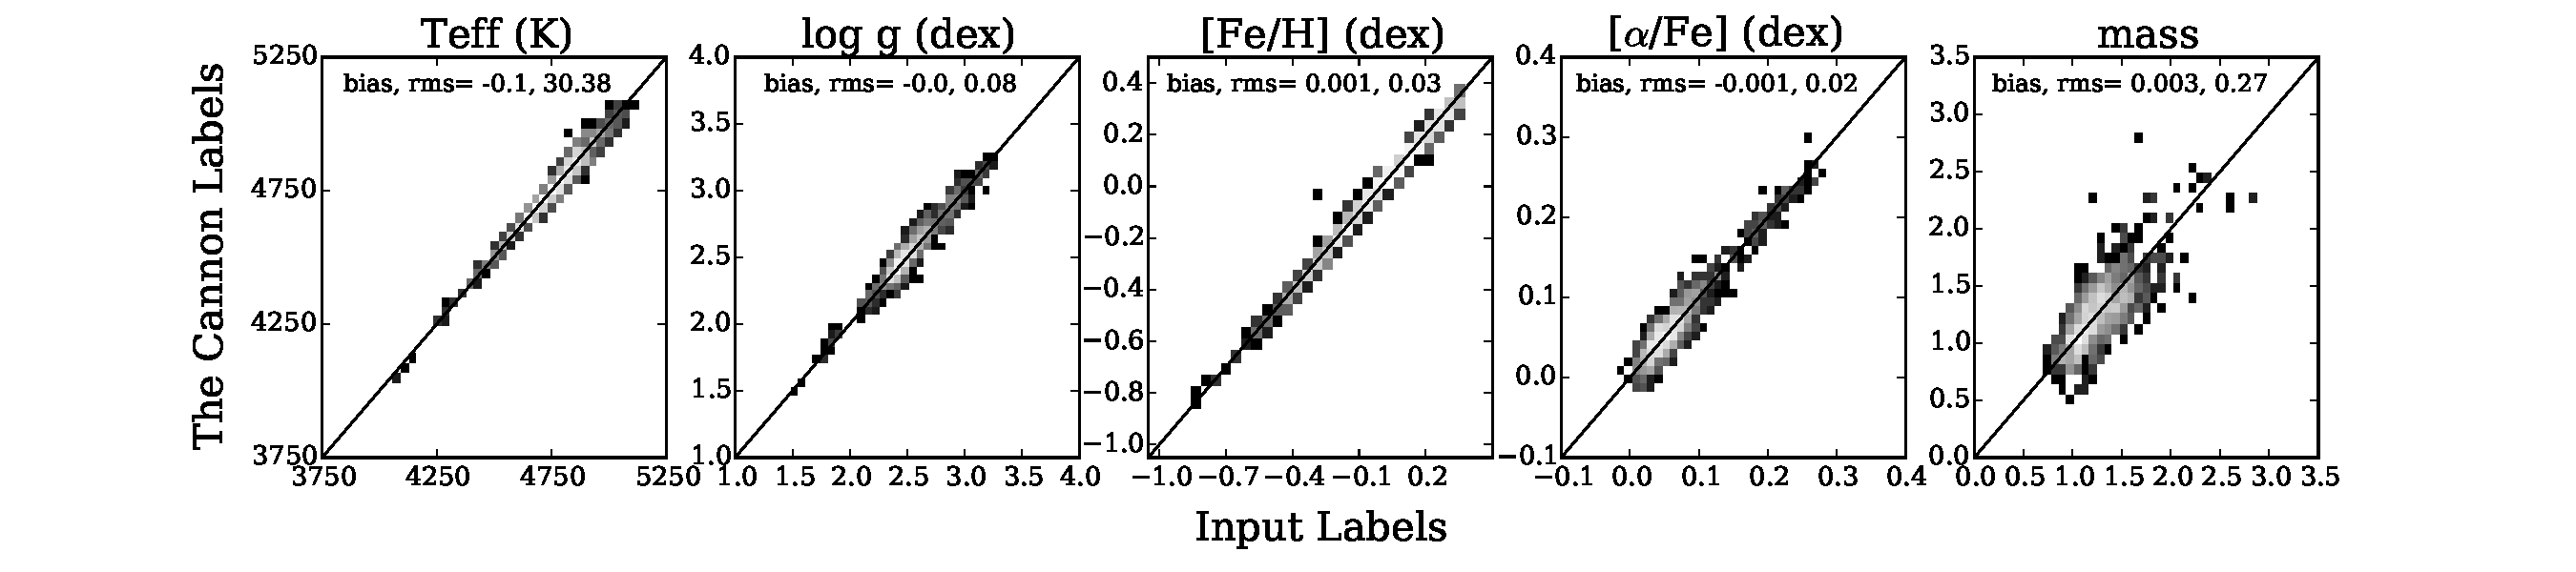
\includegraphics[scale=0.31]{./plots/validation_1500.pdf}
        \includegraphics[scale=0.35]{./plots/validation_1639_ages.pdf}
  \caption{Cross validation of training dataset for the \teff, \logg, \feh, \alphafe\ and age labels (where the mass label has been directly interpolated to mass): the results for \tc's labels for training performed on 90\% of the \apokasc\ stars, showing the performance at test time on the 10\% of the stars not included in training, run 10 times.}
\label{fig:validation2}
\end{figure}


%(note this improves by 10\,percent from 0.27 to 0.24 if take errors on nu max and delta nu to less than 5 percent. )

%from MM:\\ 
%- error on delta$\_$nu and nu$\_$max lower than 5\,percent (the cut was at 10% before)\\
%- no star in the list of fast rotating stars from Jamie Tayar\\
%- no warning or error in ASPCAPFLAG\\
%- Carbon and Nitrogen abundances $>$-9999\\
%In this way, it is only the residuals between the model and the test stars contain all of the additional information that is not already contained within the 5-labels. 
%dependency. 

\section{Experiments and results}

\subsection{Experiments and results: Interpretation of the residuals}

\tc\ is a generative model made from the set of reference objects and we can, for a given set of the five labels, produce a model spectrum of that star.  The coefficients of the model that are returned at each pixel quantify how much the label (or labels in the case of the cross-terms) describes the flux at that pixel. A near-zero coefficient for a given pixel indicates that the pixel is not described by the label/s and the largest values of the coefficients are where the spectra changes most significantly with the label or labels. 

In the following set of Figures \ref{fig:logg} to \ref{fig:mass}, we demonstrate the model coefficients and generated spectra across small wavelength regions ($\approx$ 30 Angstrom) centered on where the coefficients reach their largest amplitudes, for each of the five labels. We use the DR12 \apogee\ linelist, Kurucz model atmospheres (cite) and the stellar synthesis code MOOG (Sneden et al., 199X), to determine which elements correspond to the absorption features in the spectra where the highest coefficients are located. The absorption features in the H-band are heavily blended with OH, CN and C2 molecules and the figures indicate which absorption features are comprised of blends of molecules and elements, at the for the stellar parameter space of \apogee\ stars. The elements that show the most significant changes with the labels show a gratifying agreement with expectations from stellar physics and these are discussed below, for each of the five labels. 

Figure \ref{fig:logg} shows the 30 Angstrom regions of the spectra centered on the two highest first-order \logg\ coefficient $\theta_{logg}$. The three panels at left show the highest \logg\ coefficient and the three panels at right show the second highest coefficient. The top panel of \this Figure shows the zeroth order-coefficient vector $\theta_0$, or the baseline spectrum of the model and this is, essentially, the intersect spectrum of the training set of stars. Relevant elements and molecules that correspond to the absorption features are marked. The middle panel of Figure \ref{fig:logg} shows the first order coefficients that are linear in \teff, \logg, \feh, \alphafe\ and mass. The coefficients have all been normalised to their largest absolute value, so that an amplitude of $\theta_{ref}$ = 1 for any coefficient is at the highest value.  The bottom panel of Figure  \ref{fig:logg} shows a generated spectrum from \tc's model for a reference set of stellar parameters of a star in the training set, at \teff = 4710K, \feh = 0.05 and \alphafe = 0.015, for three different \logg values of \logg\ = 1.5, \logg\ = 2.1 and \logg\ = 3.3. From the centre left panel of Figure \ref{fig:logg} it is clear that any given pixel can have a dependency on multiple labels, and typically some coefficients, like \teff\ and \logg\ show an inverse relationship with the spectra. The Mg feature in the spectra shown in the top hand panel of Figure \ref{fig:logg} corresponds to the location of the highest amplitude \logg\ linear coefficient. The highest amplitude of this coefficient corresponds to the wings of the Mg line and not the core, in particular, the higher wavelength side of the Mg wing. The core of the Mg feature actually corresponds to a rapid decrease in the coefficient,or reduction in the information content of these pixels with respect to the \logg\ label. This Mg feature at 15770.15 Angstroms, is one of the two strongest Mg features (along with the Mg feature at 15753.29 Angstroms) across the \apogee\ H-band spectral region. The wings of strong lines are known as \logg\ indicators in stars \citep{Gray2008} and the wings of Mg lines in the optical wavelength region, which are sensitive to pressure broadening, are demonstrated in \citet{F1997} to be features from which to derive \logg\ for F and G main sequence stars. That the strongest coefficient in \logg\ comes from the wings of a strong Mg line in the H-band \apogee\ spectral region is therefore well aligned with empirical analyses in other, more comprehensively studied wavelength regions. Brackett lines (as well as Balmer and Paschen lines)  are similarly sensitive to pressure (Stark) broadening and are therefore excellent tracers of \logg\ in stars. The second highest amplitude coefficient is at the Brackett feature in the \apogee\ spectral region and the bottom panel at right shows how significantly the flux varies as a function of \logg\ for the Brackett feature at $\apprx$ 16810 Angstroms. In addition to being second highest in amplitude, the sign of this coefficient for this feature is positive and so has the opposite relation with flux to that of the \logg\ parameter and the Mg wings. As seen in the bottom panel at left, the wings of the Mg feature deepen with increasing \logg, where as for the Brackett feature at right, the spectral profile flattens with increasing \logg, for any given set of stellar \teff, \feh, \alphafe\ and mass parameters, hence the inverse relative relationship between the two features. 

Figure \ref{fig:teff} shows the same information as Figure \ref{fig:logg} but for the two highest \teff\ coefficients, centered on $\approx$ 15338 and 15720 Angstroms. The highest \teff\ coefficients correspond to the core of two Ti lines in the spectra (one of which is blended also with Fe and the other with CN). The temperature coefficient is in typically positive in the \apogee\ spectral region, with exceptions, for example at the Brackett feature shown in Figure \ref{fig:logg} )where it is inversely correlated with the \logg\ coefficient). \teff\ is typically strongly anticorrelated with \feh\ and \alphafe as seen in Figure \ref{fig:teff}: in a spectra at a given \feh, as the temperature increases the lines weaken and so the flux decreases, similarly, at a given \teff, as the metallicity increases the lines strengthen, and the flux increases. That we have coefficients for features that we can directly identify from the \apogee\ linelist means that, we have a model not only for the (typically blended) absorption features, but how all of the individual elements behave with the five modeled labels at the limit of the spectral resolution. For example, note the asymmetry in the behaviour of the variation of the \teff\ label for the spectra in the left bottom panel of Figure \ref{fig:teff}: this reflects the blending of the absorption feature and that coefficients at a given flux are sensitive to  particular individual elements rather than particular absorption features. It is possible to describe this only with  coefficients that are determined at every wavelength in flux. 

Figure \ref{fig:feha} is demonstrative of the highest \feh\ and \alphafe\ coefficient in the spectra. The \feh\ and \alphafe\ labels are typically correlated with the cores of all of the absorption features in the spectra, particularly for the \feh\ label, as seen at left. The [M/H] of  a star simply correlates with the \feh\ and the \alphafe\ is known to increase with \feh\ and flatted to a plateau at high \alphafe and low \feh, subject to the star formation rate and initial mass function. For many but by no means all absorption features, the \teff\ shows an inverse correlation with temperature as seen in the left hand panel of Figure \ref{fig:teff}. The strongest \feh\ coefficient corresponds to a core of a (blended) Mn feature, the flux of which changes dramatically as a function of \feh\ over the range of \feh = --0.8 -- +0.2 as shown in the bottom panel of Figure \ref{fig:teff}. Mn is one of the Fe-group elements (in addition to V, Ti, Cr, Co and Ni) this element correlates directly with \feh\ \citep[see][]{Maria2008, B2015}. The largest coefficient in \alphafe\ corresponds to the core of the strong Mg line at $\approx$ 16370 Angstroms (also belnded with CO and OH) and dissimilarly to the \logg coefficent, it is the core of the line that correlates with \alphfe\. Note that for the \logg\ coefficient at this blended Mg feature in the middle panel of Figure \ref{fig:feha} at right that the \logg\ coefficient is $\approx$ 0 at the very centre of the line profile and increases to a significant dependency in the wings of the feature, primarily for the higher wavelength edge. 



, this relationship may break down for more metal-poor stars \feh\ $<$ --1.0. 


For the first label vector for example in the middle panel of \figurename~\ref{fig:coeffs}, 
there is typically asymmetry for a given absorption feature, in the flux and the labels. 
There are very few regions where the flux is a function of only one of the labels, and pixels are typically co-variant. 
(that is, the same pixel will have a higher flux at both lower \teff\ and higher \feh). 
This simply reflects well-known co-variances between, for example, temperature and \feh .
The strongest \logg\ dependence is typically associated with weak lines including the wings of the 
feature and the \feh\ label, with strong lines, particularly the depth of the line. 

The bottom panel of \figurename~\ref{fig:coeffs} shows the scatter vector of the spectral model, 
indicating the dispersion of the flux of the training data around the best-fit spectral model at each pixel. 
The scatter is small and this indicates that our model is a good representation of the data. 
However, the scatter is highest where the most information in the spectra are contained. 
This implies that either our quadratic-in-labels spectral model is still somewhat too restricted, or that the labels of our training dataset are imperfect or incomplete 
(for example, lacking $[\alpha / Fe]$ as a label), or a combination of these effects. 
From the coefficients of an initial fit of this spectral models (see, for example, the middle panel of \figurename~\ref{fig:coeffs}), 
the continuum pixels have been determined following \sectionname~\ref{sec:ContNorm}. 
These are marked in the cyan dots in the top panel of the \figurename, and are used for an iterated, 
consistent continuum-normalization for all spectra, both of the reference and of the survey objects.

% run run -i makeplot_scatter_test18_step/spectra in /Apogee_ages/ o
\begin{figure}[p!]
\centering
 % \includegraphics[scale=0.31]{./plots/validation.png}
    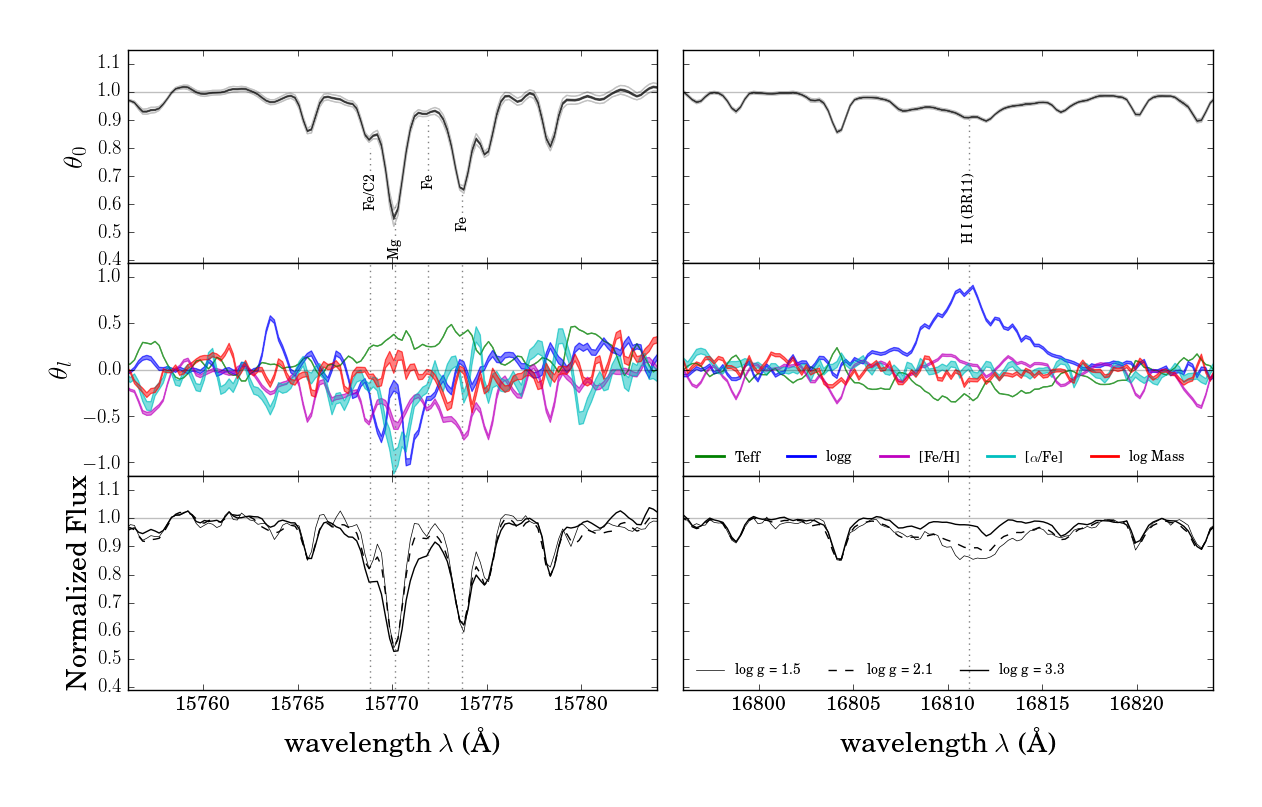
\includegraphics[scale=0.51]{./plots/coeffs_g_3.png}
  \caption{The first order coefficients of the model trained on the \aspcap\ stars showing the two 20 Angstrom wavelength regions where the \logg\ coefficient reaches the highest absolute amplitude. The 0th coefficient (at top) describes the intersect spectrum and relevant spectral absorption features are marked. The lower panel shows all coefficients, each normalised to their highest amplitude, for all \teff, \logg, \feh,\alphafe\ and mass coefficients.}
\label{fig:logg}
\end{figure}

Figure \ref{fig:g} shows the two 20 Angstrom regions where the \logg\ coefficient reaches the highest amplitude. The intersect spectra (0th coefficient) is plotted at top and the coefficients for the 5 labels are plotted in the bottom panels.  The left panel includes some of the elements corresponding to the absorption lines. The IR spectral region is highly blended with molecular features and most lines are a blend including CN, C2 and OH features. The maximum amplitude of the \logg\ coefficient does not correspond to the core of the absorption feature of the intersect spectrum but rather the wings. As \logg\ increases, these wings broaden and deepen. Consersely, the panel on the right hand side is the second highest amplitude of the \logg\ coefficient but is positive, The feature this correlates with is the Brackett feature, which becomes shallower and flatter with increasing \logg. 




\subsubsection{Teff residuals}

The strongest \teff residual is at 15720 \AA. 

% run run -i makeplot_scatter_test18/spectra_step in /Apogee_ages/ o
\begin{figure}[p!]
\centering
 % \includegraphics[scale=0.31]{./plots/validation.png}
    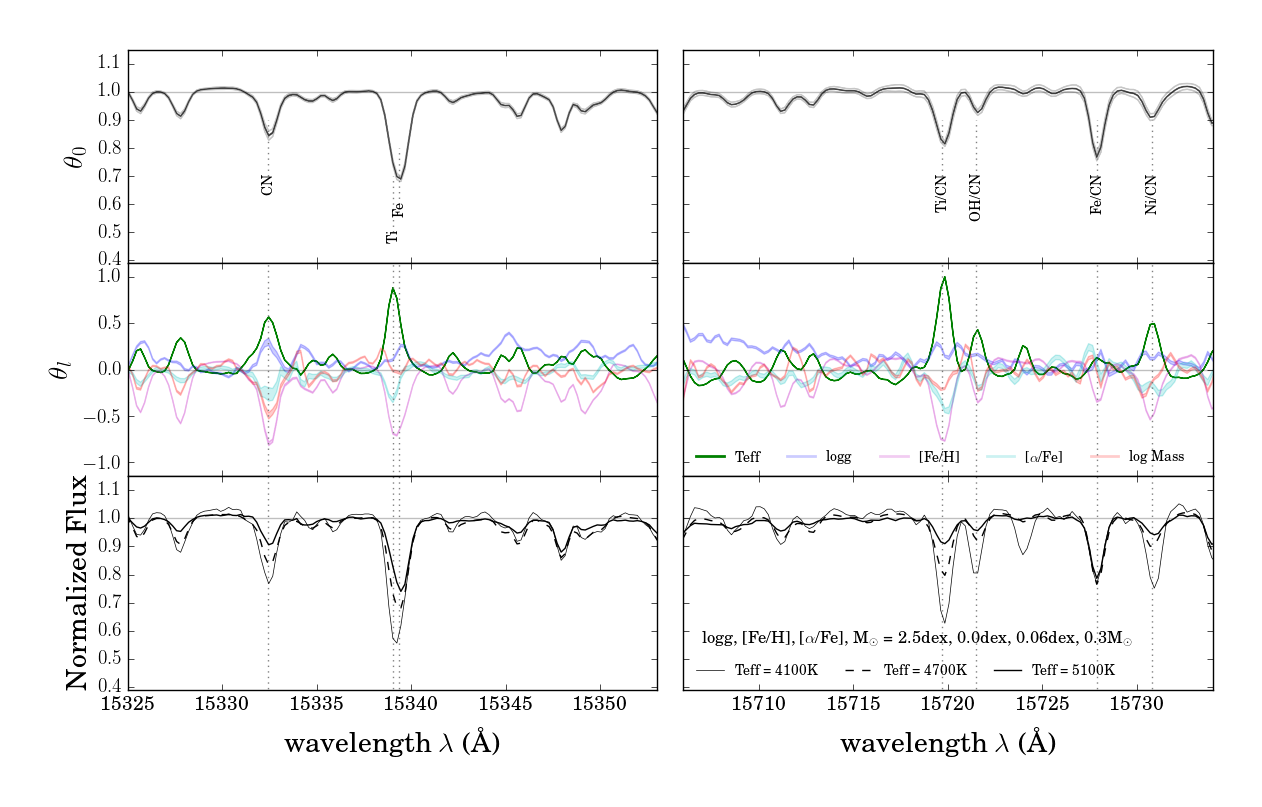
\includegraphics[scale=0.51]{./plots/coeffs_t_3.png}
  \caption{The first order coefficients of the model trained on the \aspcap\ stars showing the two 20 Angstrom wavelength regions where the \teff\ coefficient reaches the highest absolute amplitude. The 0th coefficient (at top) describes the intersect spectrum and relevant spectral absorption features are marked. The lower panel shows all coefficients, each normalised to their highest amplitude, for all \teff, \logg, \feh,\alphafe\ and mass coefficients.}
\label{fig:teff}
\end{figure}

This is a Ti I line. \\

% run run -i makeplot_scatter_test18_step_spectra in /Apogee_ages/ o
\begin{figure}[p!]
\centering
 % \includegraphics[scale=0.31]{./plots/validation.png}
    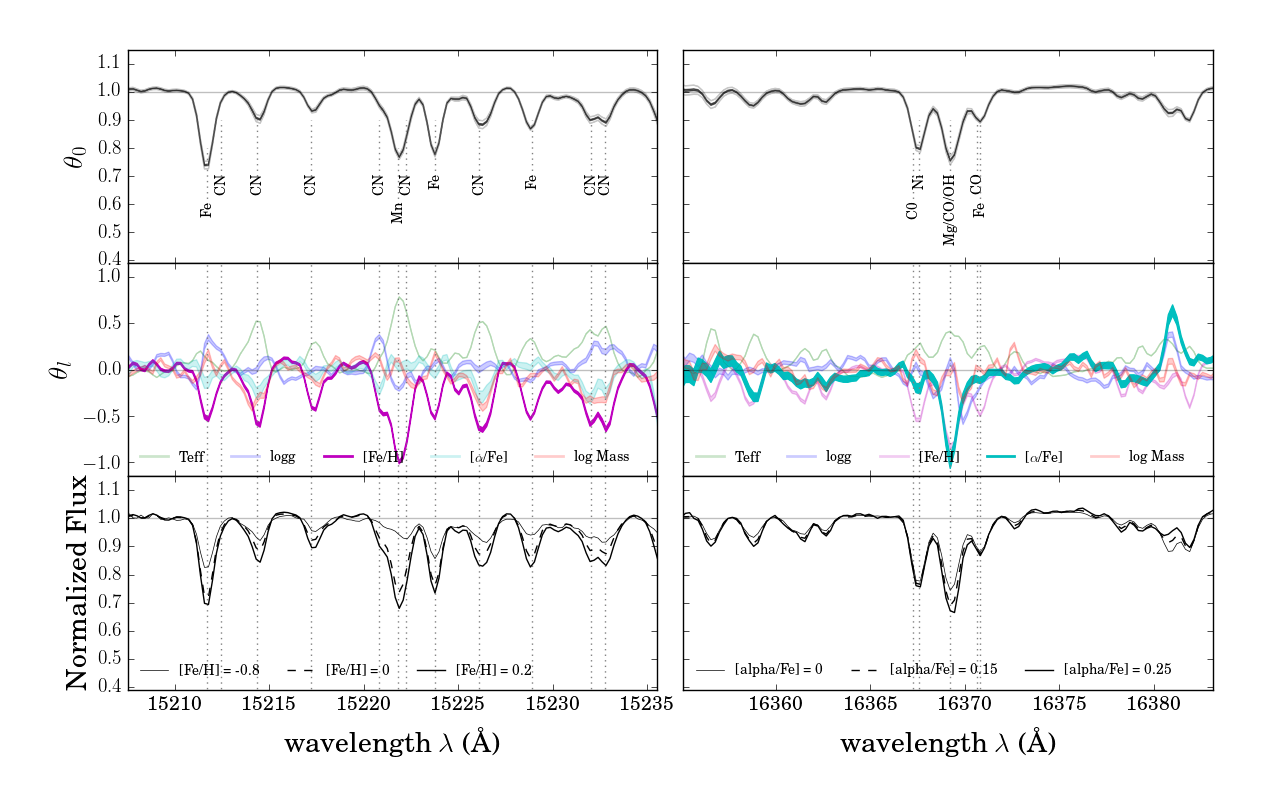
\includegraphics[scale=0.51]{./plots/coeffs_af_3.png}
  \caption{The first order coefficients of the model trained on the \aspcap\ stars showing the two 20 Angstrom wavelength regions where the \teff\ coefficient reaches the highest absolute amplitude. The 0th coefficient (at top) describes the intersect spectrum and relevant spectral absorption features are marked. The lower panel shows all coefficients, each normalised to their highest amplitude, for all \teff, \logg, \feh,\alphafe\ and mass coefficients.}
\label{fig:teff}
\end{figure}

\begin{figure}[p!]
\centering
 % \includegraphics[scale=0.31]{./plots/validation.png}
    
\includegraphics[scale=0.51]{./plots/coeffs_m_3.png}
  \caption{The second coefficient is not there if train on linear mass - concerning..}
\label{fig:feha}
\end{figure}'



%run -i makeredclumpplot.py
\begin{figure}[p!]
\centering
 % \includegraphics[scale=0.31]{./plots/validation.png}
     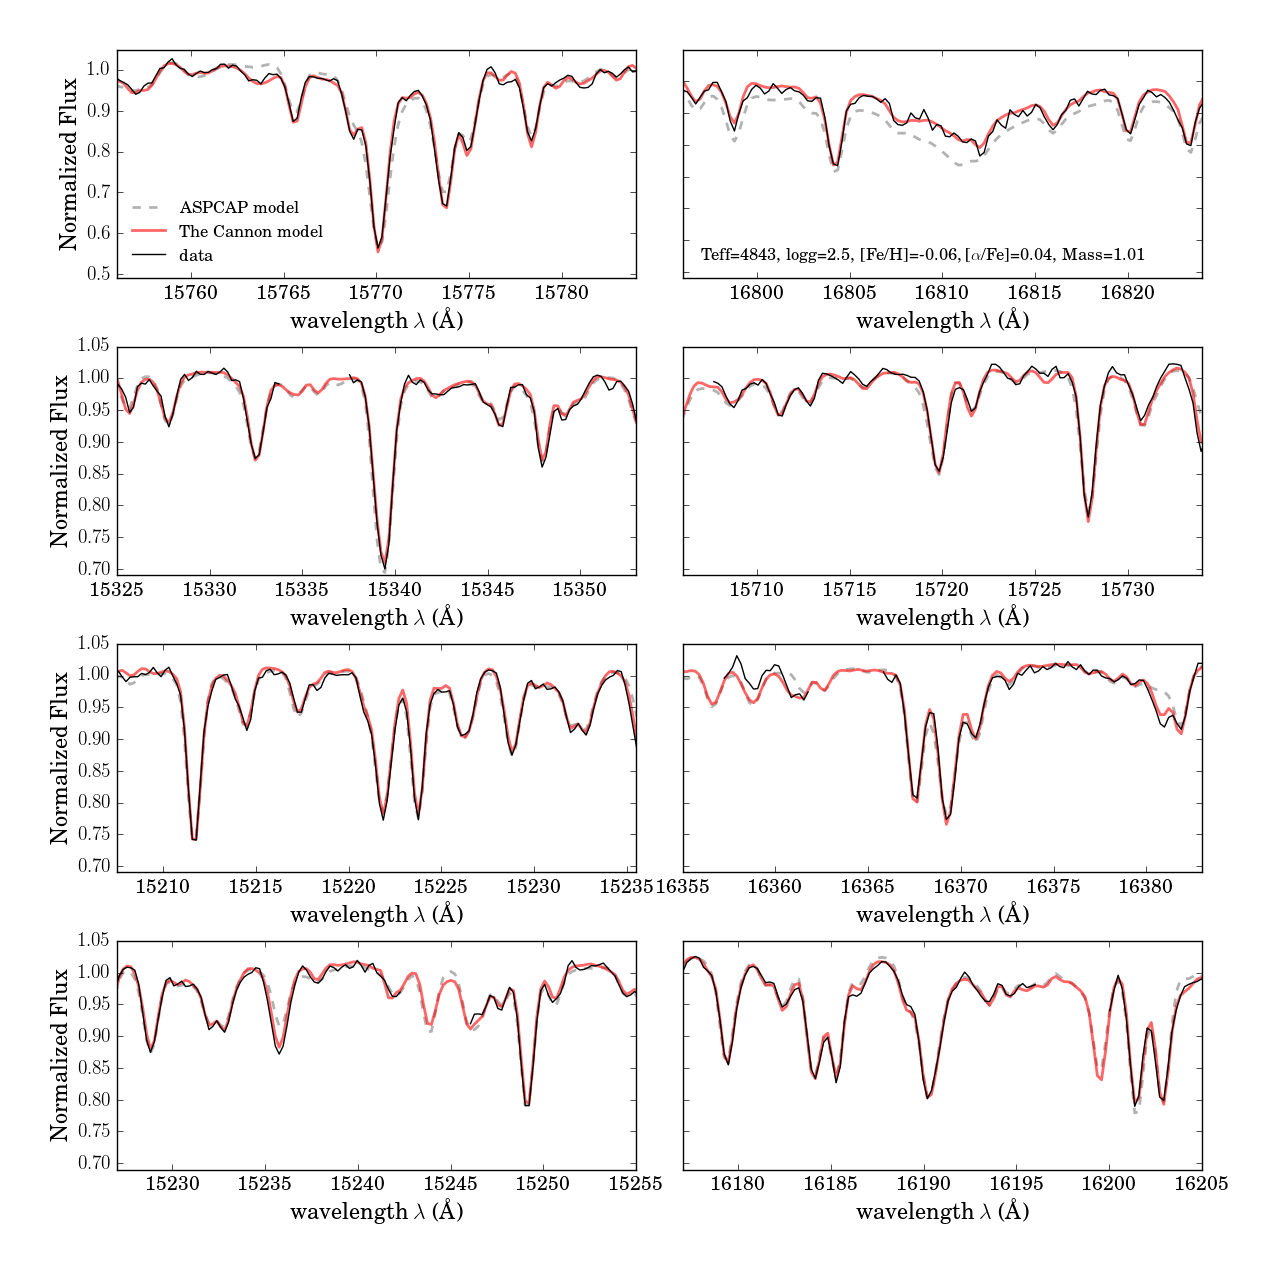
\includegraphics[scale=0.5]{./plots/spectra_fits_7.png}
%    \includegraphics[scale=0.5]{./plots/spectra_fits_7_tg.png}\\
%    \includegraphics[scale=0.5]{./plots/spectra_fits_7_fm.png}
  \caption{fits in regions of logg and teff at top and feh and alphafeh and mass at bottom.}
\label{fig:mass}
\end{figure}





\ldots MKN: how do we show that we are simply not reproducing the alpha-\feh\ information:

\section{Kepler sample  - validation age is meaningful} 

% made in makealphamap3.py  in Apogee_ages after running plotdiff_5labels2
% run -i /Users/ness/new_laptop/Apogee_ages/makealphamap4_logmass.py
\begin{figure}[p!]
\centering
 \includegraphics[scale=0.45]{./plots/alpha_feh_bins3.pdf}
    \caption{The \feh-\alphafe\ plane colored by mean age of the stars in each bin. The number of stars in each bin is indicated }
\label{fig:alphabins}
\end{figure}

\begin{figure}[p!]
\centering
 \includegraphics[scale=0.45]{./plots/alpha_feh_std3.pdf}
    \caption{The \feh-\alphafe\ plane colored by standard deviation of the age of the stars in each bin. The number of stars in each bin is indicated }
\label{fig:alphabins}
\end{figure}

% made in makealphamap4_logmass.py after running the plotdiff as above
\begin{figure}[p!]
\centering
 \includegraphics[scale=0.45]{./plots/Kepler_Cannon_diff.pdf}
    \caption{The stars in Figure 8 individually subtracted from the mean age in their respective bin, showing correlation within the individual mono-abundance bins in the \alphafe-\feh\ plane. }
\label{fig:alphabins}
\end{figure}

\section{Red clump sample - some results } 

%run -i makealphafeh_imshow_3panel.py and readin_ages.py
\begin{figure}[p!]
\centering
 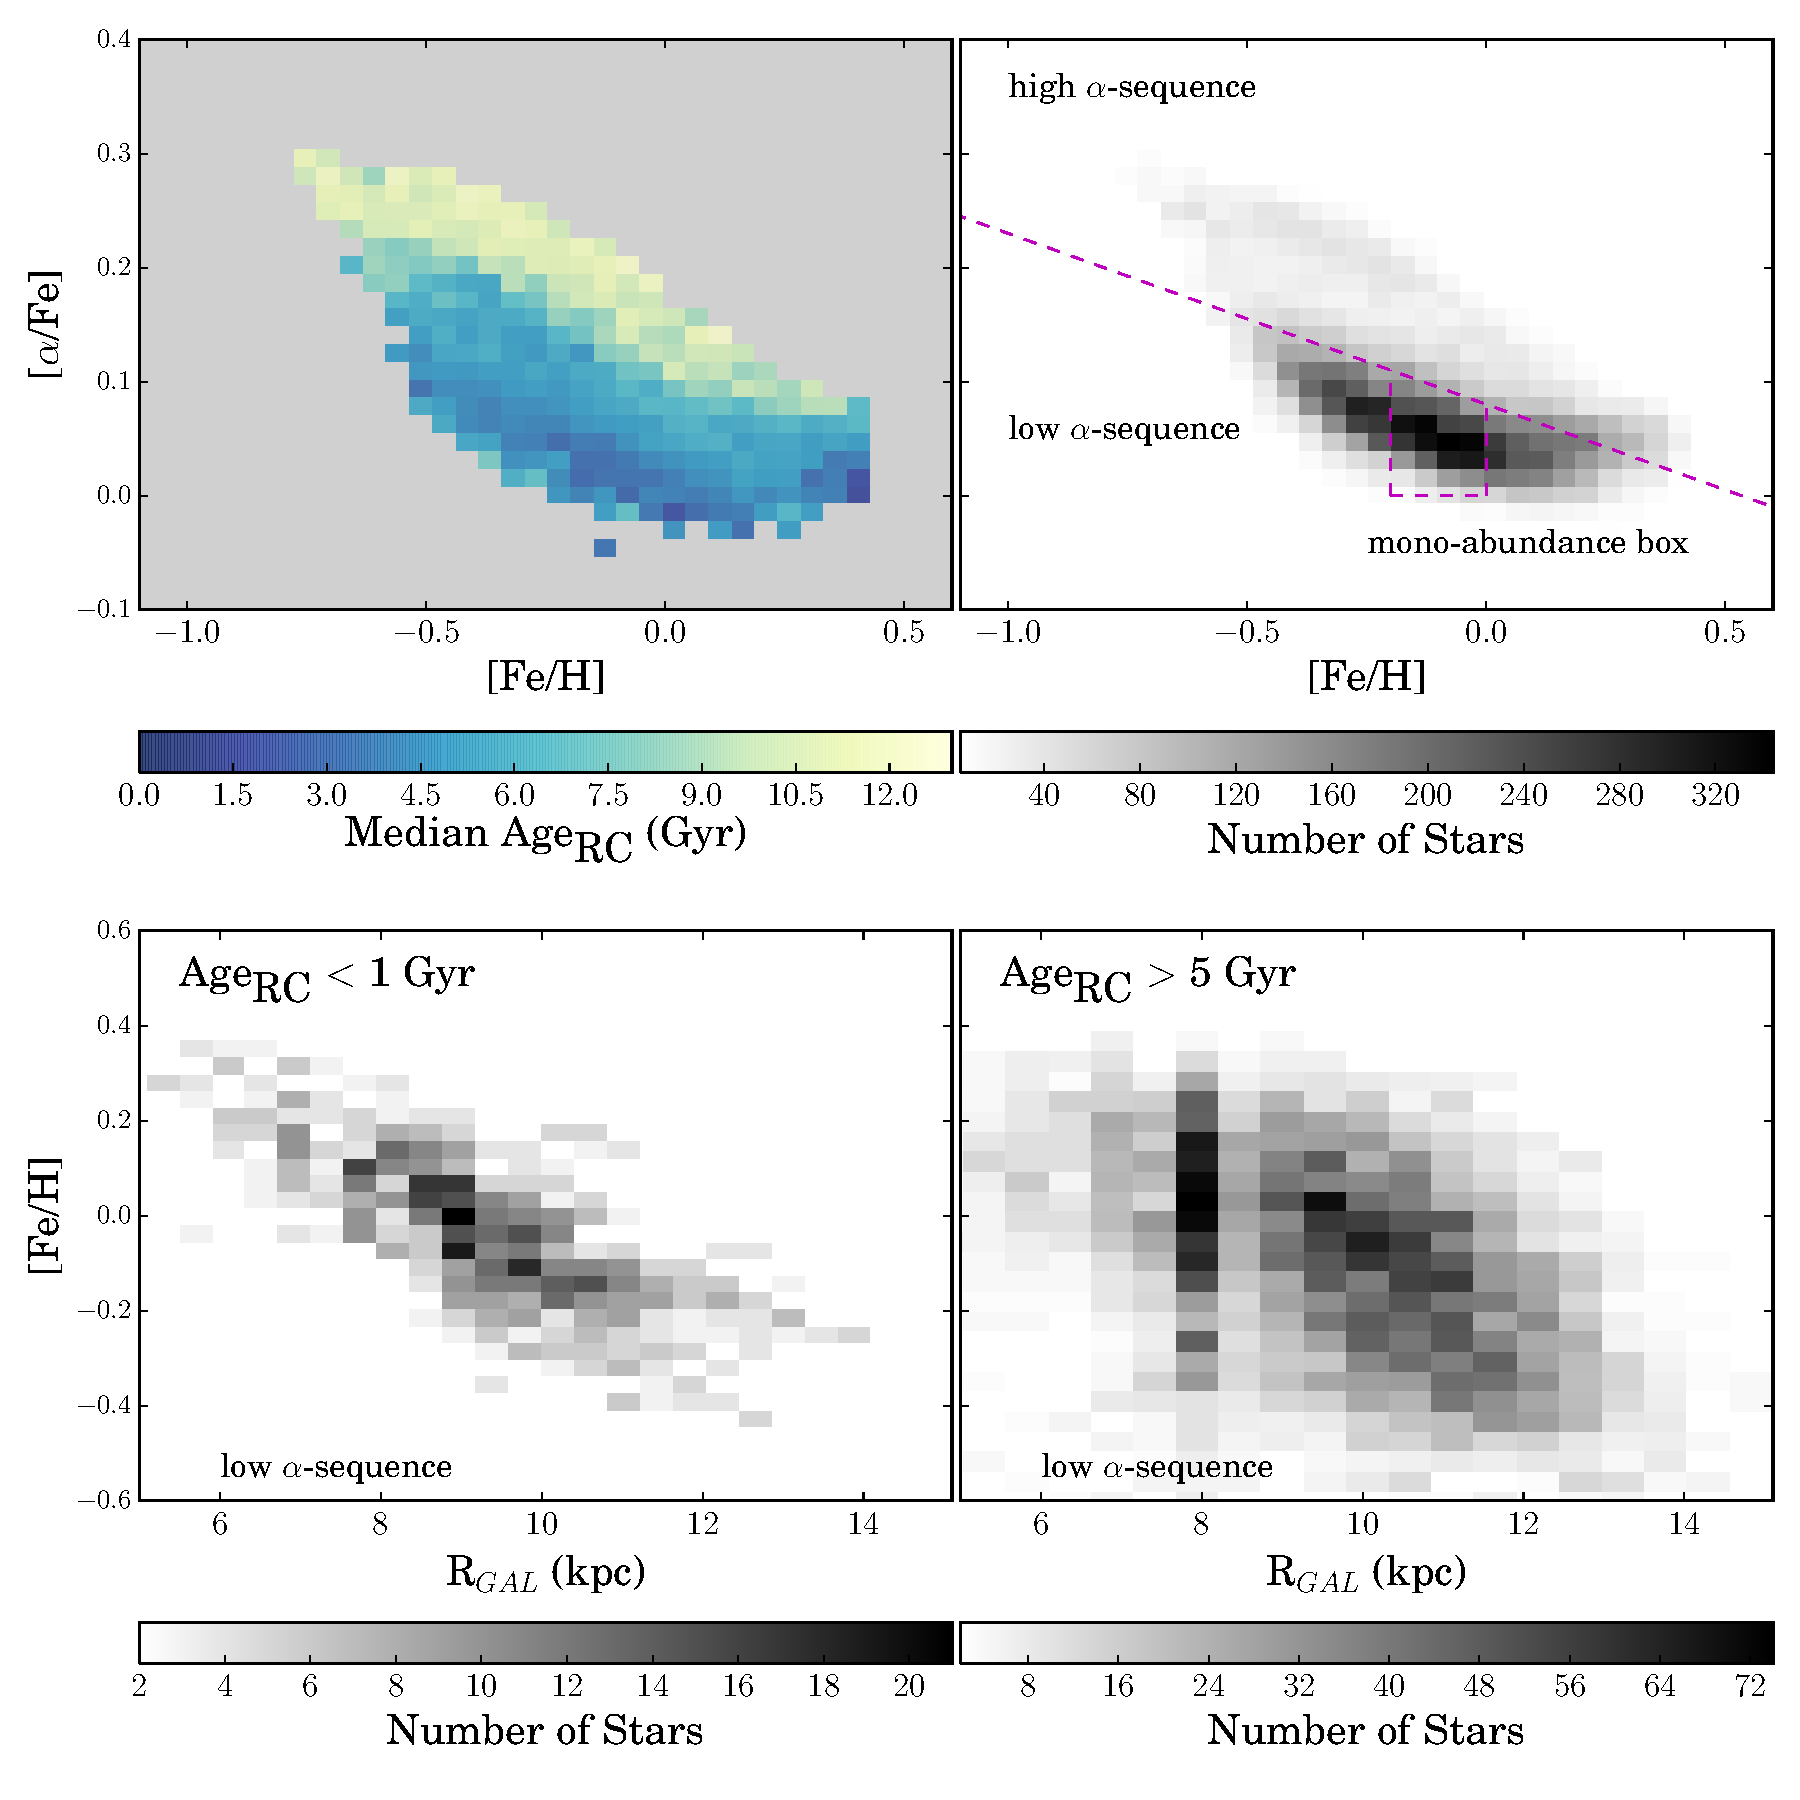
\includegraphics[scale=0.4]{./plots/redclump_4panel.pdf}
    \caption{The 20K red clump sample: low alpha sequence is broken up into radius and box is the mono-abundance distribution in later figure.}
\label{fig:alphabins}
\end{figure}

% made in /Users/ness/new_laptop/Apogee_ages/dwh/makeplots_mkn.py 
\begin{figure}[p!]
\centering
 % \includegraphics[scale=0.31]{./plots/validation.png}
    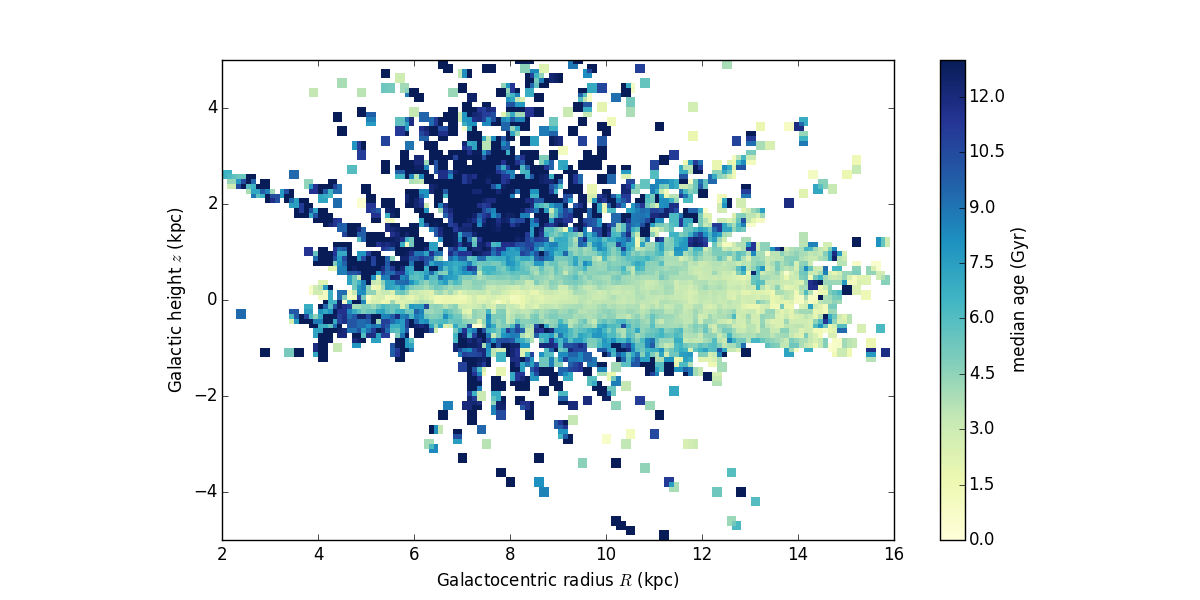
\includegraphics[scale=0.45]{./plots/median_age_abs.png}
    \caption{The median age of the 20,000 red clump stars  }
\label{fig:alphabins}
\vspace{360pt}
\end{figure}

% made in /Users/ness/new_laptop/Apogee_ages/dwh/makeplots_mkn.py 
\begin{figure}[p!]
\centering
 % \includegraphics[scale=0.31]{./plots/validation.png}
    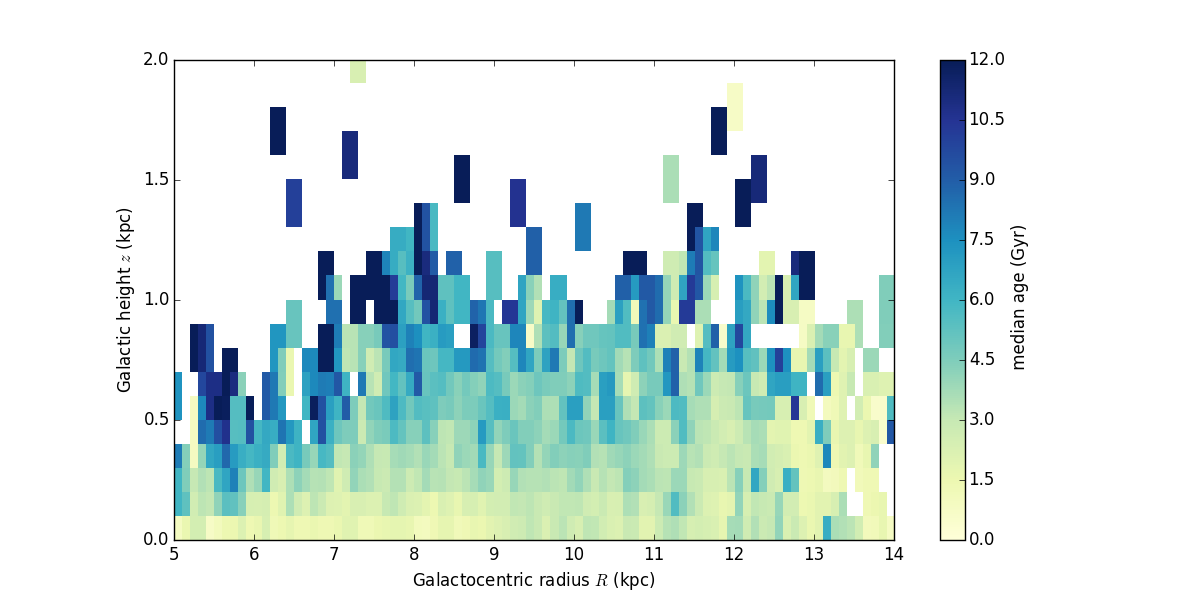
\includegraphics[scale=0.45]{./plots/median_age_low_alpha_abs.png}
    \caption{The median age of the low alpha sequence of the red clump stars ( draw where this in in feh alphafeh plane). Include number of stars. }
\label{fig:alphabins}
\vspace{-30pt}
\end{figure}

% made in /Users/ness/new_laptop/Apogee_ages/dwh/makeplots_mkn.py 
\begin{figure}[p!]
\centering
 % \includegraphics[scale=0.31]{./plots/validation.png}
    \includegraphics[scale=0.45]{./plots/median_age_mono_abs.png}
    \caption{The median age of low alpha sequence monoabundance  bin with a cut on  \feh\ of 0 to -0.2. }
\label{fig:alphabins}
\end{figure}

%\begin{figure}[p!]
%\centering
% % \includegraphics[scale=0.31]{./plots/validation.png}
%    \includegraphics[scale=0.3]{./plots/median_age_high_alpha_abs.png}
%    \caption{median age of high alpha sequence = draw where this in in feh alphafeh plane. }
%\label{fig:alphabins}
%\end{figure}

\ldots MKN: What are the spectral signatures of mass and how do they
map on to our hypothesized mass and age indicators?


\ldots MKN: What does the Galaxy look like in terms of age gradients,
in subsamples chosen for chemical homogeneity?

\section{Discussion}

\ldots DWH: Re-cap of what we have achieved and how we know we have
succeeded.

\ldots DWH: Emphasis on the reason that the science result is so
convincing that we really have an age indicator here.

\ldots MKN: What of the hypothesized age indicators are in fact
dominant?

\ldots MKN: How do you obtain our code, data, and results?

\acknowledgments
It is a pleasure to thank
  Foo,
  John Bochanski (Rider),
  Dan Foreman-Mackey (UW), and
  Bar,
for valuable discussions and contributions.
This project made use of
  The NASA Astrophysics Data System,
  and open-source code in the \project{numpy} and \project{scipy} packages.

[Insert SDSS boilerplate here.]

All code and data produced in this project is available HERE and THERE.

\bibliography{tc.bib}

\end{document}
